%----------------------------------------------------------------------------------------
%	PACKAGES AND THEMES
%----------------------------------------------------------------------------------------

\documentclass[11.5pt, aspectratio=169]{beamer} %handout

\usepackage{Style/style}

%----------------------------------------------------------------------------------------
%	TITLE PAGE
%----------------------------------------------------------------------------------------

% The short title appears at the bottom of every slide, the full title is only on the title page
\title[]{Recent Advances In Document-level Neural Machine Translation} 

\author[L.\,Lupo]
{%
  \texorpdfstring{
    \begin{columns}%[onlytextwidth]
      \column{1\linewidth}
      \centering
      Lorenzo Lupo\\
      \medskip
      Supervisors: Laurent Besacier, Marco Dinarelli\\
    \end{columns}
  }
  {Lorenzo Lupo}
}
		 
%\institute[Polimi] % Your institution as it will appear on the bottom of every slide, may be shorthand to save space
{%
%Politecnico di Milano%\\ % Your institution for the title page
%\medskip
%\textit{john@smith.com} % Your email address
}


\begin{document}

\begin{frame}[plain]
%	\begin{figure}[htpb]
%		\centering
%		\includegraphics[width=0.3\linewidth]{Images/polimi}
%	\end{figure}
	\titlepage
\end{frame}

%------------------------------------------------------------------------------
% Introduzione 
%------------------------------------------------------------------------------


\begin{frame}{What is Document-level Machine Translation}
	\begin{figure}
	\centering
	\begin{minipage}{.4\textwidth}
		\centering
		\textbf{Sentence-level MT}\par\medskip
		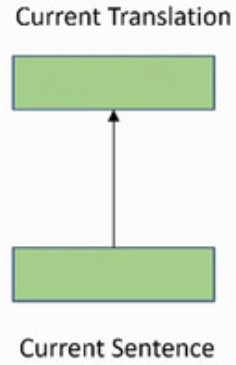
\includegraphics[width=.4\linewidth]{Images/dlmt}
	\end{minipage}%
	\begin{minipage}{.6\textwidth}
		\centering
		\textbf{Document-level MT}\par\medskip
		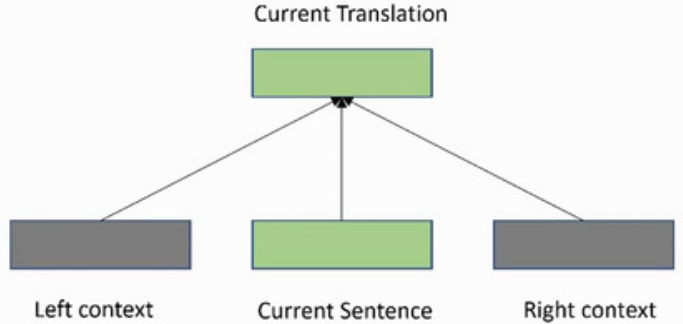
\includegraphics[width=.85\linewidth]{Images/slmt}
	\end{minipage}
	\end{figure}	
\end{frame}

\begin{frame}{Document-level MT $\leftrightarrow$ Context-aware MT}
	\begin{figure}
	\centering
	\begin{minipage}{.4\textwidth}
		\centering
		\textbf{Context-agnostic MT}\par\medskip
		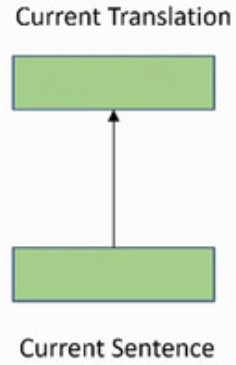
\includegraphics[width=.4\linewidth]{Images/dlmt}
	\end{minipage}%
	\begin{minipage}{.6\textwidth}
		\centering
		\textbf{Context-aware MT}\par\medskip
		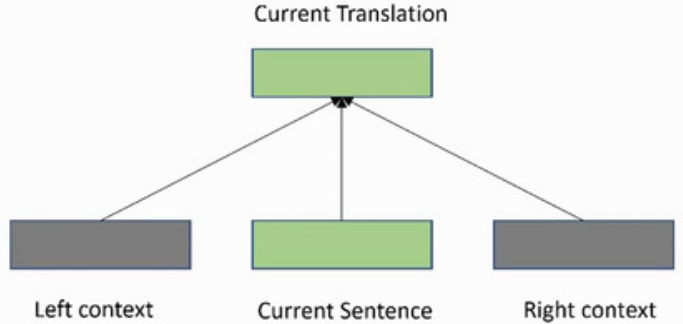
\includegraphics[width=.85\linewidth]{Images/slmt}
	\end{minipage}
	\end{figure}	
\end{frame}

\begin{frame}{Why Document-level NMT ?}
	
	\begin{itemize}
		\item<+(1)-|alert@+(1)>{Some recent results suggest that neural machine translation (NMT) "approaches the accuracy achieved by average bilingual  human  translators  [on  some  test  sets]” \cite{wu_googles_2016}
		}
		
		\item<+(1)-|alert@+(1)>{"In a pairwise ranking experiment, human raters assessing \textbf{adequacy} and \textbf{fluency} show a stronger preference for human over machine translation when evaluating documents as compared to isolated sentences." \cite{laubli_has_2018}
		}
	\end{itemize}
	
	
\end{frame}

\begin{frame}{Sentence-level NMT is inconsistent}
	\begin{center}
		\onslide<3->{%
			\begin{minipage}{0.75\textwidth}
				\RaggedRight
				\textbf{A}: Good Morning, \textcolor{blue}{Mr. President}.
			\end{minipage}
			\bigskip
		}
		\onslide<1->{%
			\begin{minipage}{0.75\textwidth}
				\RaggedRight
				\textbf{B}: How are \textcolor{blue}{you} today?
			\end{minipage}
			\bigskip
		}
		\onslide<2->{%
			\textbf{SENTENCE-LEVEL TRANSLATION}
			\medskip
			
			\begin{minipage}{0.75\textwidth}
				\RaggedRight
				\textbf{B}: Comment \textcolor{red}{vas-tu} aujourd'hui ?
	
			\end{minipage}
			\bigskip
		}
		\onslide<4->{%
			\textbf{DOCUMENT-LEVEL TRANSLATION}
			\medskip
			
			\begin{minipage}{0.75\textwidth}
				\RaggedRight
				\textbf{B}: Comment \textcolor{green}{allez-vous} aujourd'hui ?
			\end{minipage}
		}
	\end{center}
\end{frame}

\begin{frame}{How frequent are inconsistencies ?}
	\onslide<1->{%
		\cite{voita_when_2019} undertake a  human  study  on context agnostic translation :
			\begin{itemize}
				\item 2000 pairs of consecutive English sentences (S1 + S2) from OpenSubtitles2018
				\item translate to Russian with Transformer model \cite{vaswani_attention_2017}
			\end{itemize} 
	} 
	\onslide<2->{
	\begin{figure}
		\centering
		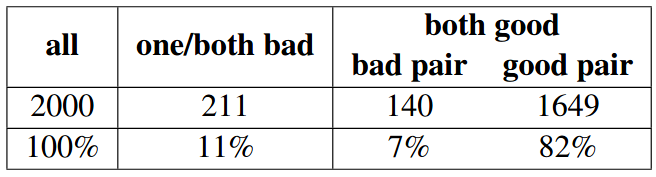
\includegraphics[width=0.7\linewidth]{Images/inconsistent_sentences}
		\label{fig:inconsistentsentences}
	\end{figure}
	}
	
\end{frame}

\begin{frame}{Which kind of inconsistencies?}
	\begin{figure}
		\centering
		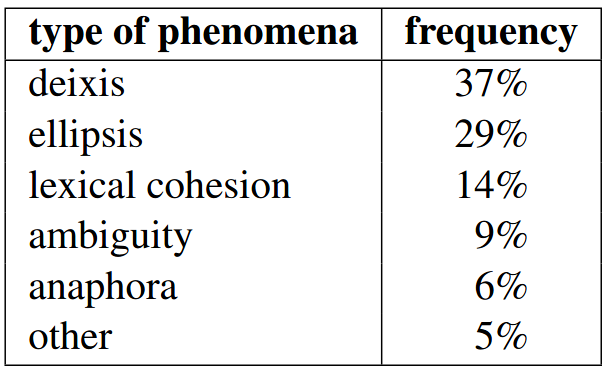
\includegraphics[width=0.7\linewidth]{Images/phenomena}
		\caption{Types of phenomena causing inconsistencies between English-Russian context-agnostic  translations  of  consecutive  sentences when placed in the context of each other.}
		\label{fig:phenomena}
	\end{figure}	
\end{frame}

\begin{frame}{Objectives}
	\begin{itemize}
		\item<+(1)-|alert@+(1)> \textbf{Design translation models and learning techniques} that solve inconsistencies by taking context into account;
		\item<+(1)-|alert@+(1)> \textbf{Evaluate such models} in a proper way;
	\end{itemize}
\end{frame}


%------------------------------------------------------------------------------
% Indice 
%------------------------------------------------------------------------------

\begin{frame}
\frametitle{Plan} % Table of contents slide, comment this block out to remove it
\tableofcontents % Throughout your presentation, if you choose to use \section{} and \subsection{} commands, these will automatically be printed on this slide as an overview of your presentation
\end{frame}

%------------------------------------------------------------------------------
% Corpo della presentazione 
%------------------------------------------------------------------------------

%\section{Approaches to DNMT}

\begin{frame}{DNMT architectures}

	DNMT architectures are based on traditional encoder-decoder models:
	
	\onslide<2->{\begin{figure}
		\centering
		\textbf{RNN-based} (until 2017)\par\medskip
		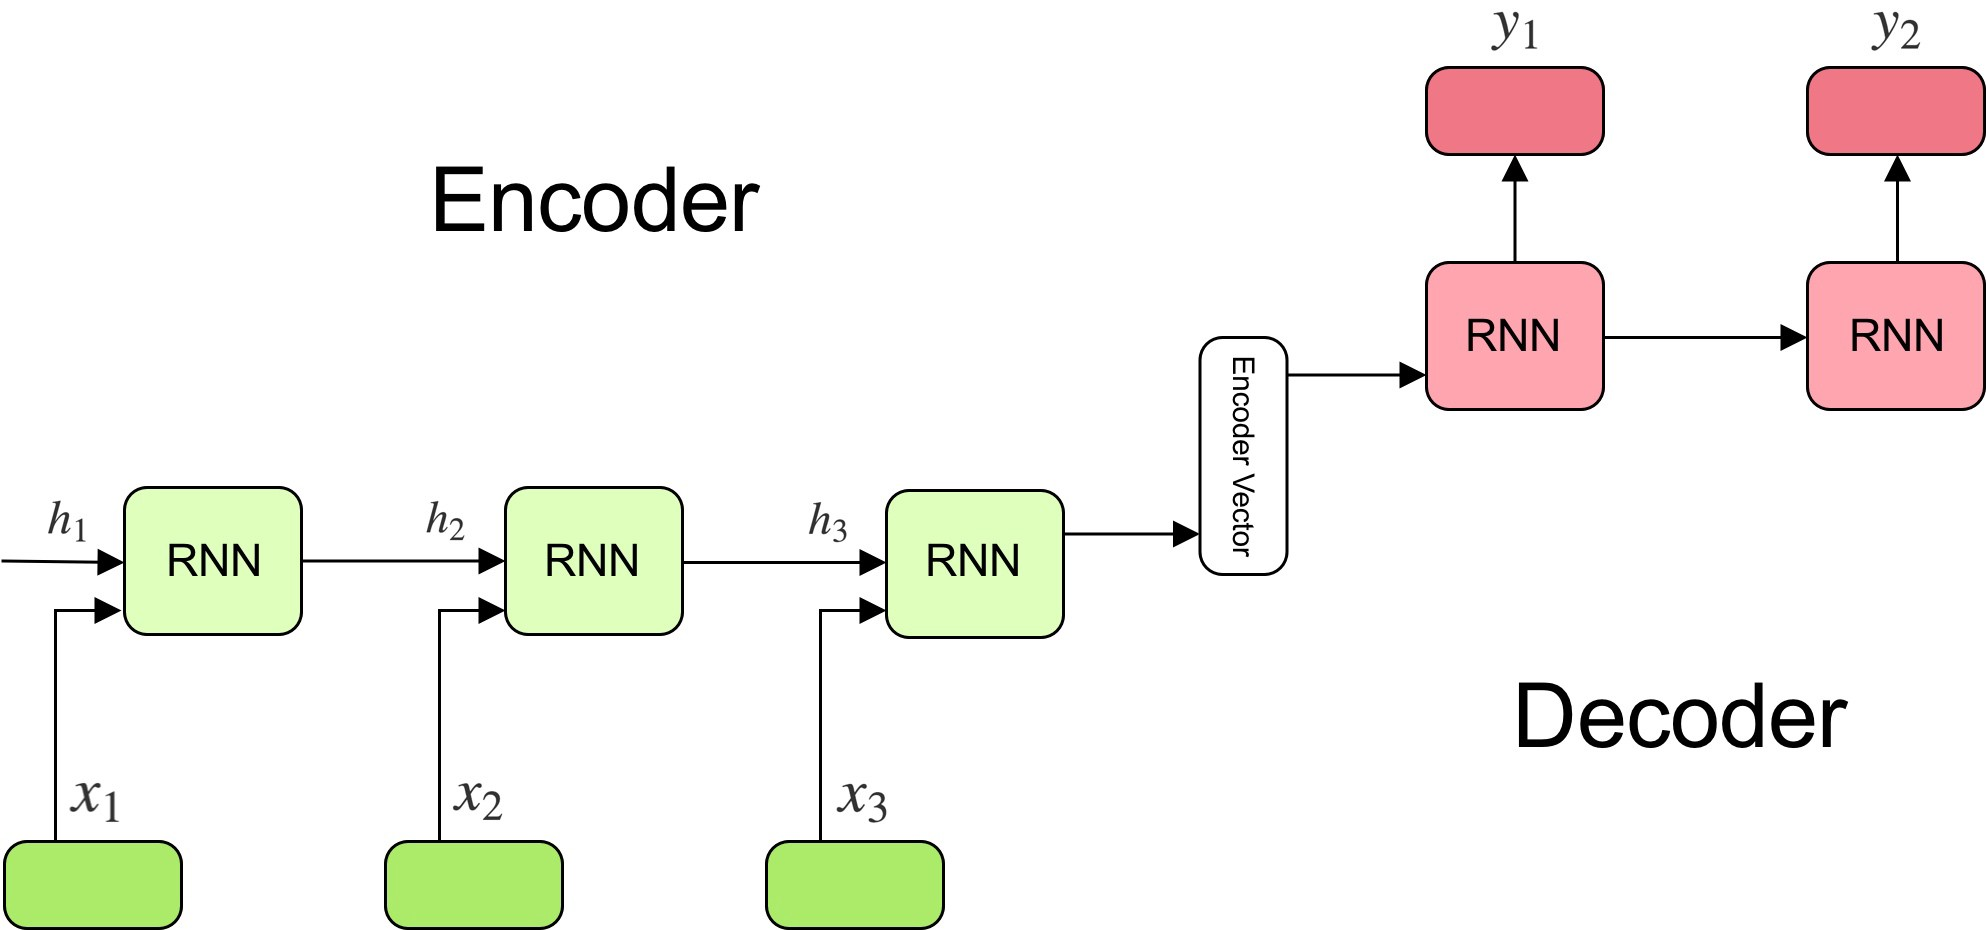
\includegraphics[width=0.45\linewidth]{Images/encoder_decoder}
		\label{fig:concatenation}
	\end{figure}
	}
\end{frame}

\begin{frame}{DNMT architectures}
	
	DNMT architectures are based on traditional encoder-decoder models:
	
	\begin{figure}
		\centering
		\textbf{Transformer-based} (afterwards)\par\medskip
		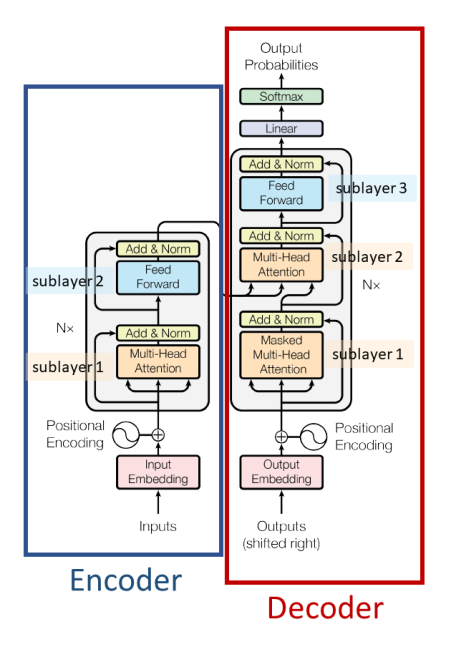
\includegraphics[width=0.3\linewidth]{Images/transformer}
		\label{fig:concatenation}
	\end{figure}
\end{frame}

%%%%%%%%%%%%%%%%%%%%%%%%%%%%%%%%%%%%%%%%%%%%%%%%%%%%%%%%%%%%%%%%%%%%%%%%%
\subsection{Concatenation Approaches}

\begin{frame}{Concatenation Approaches}
Concatenation approaches to DNMT consist in feeding a standard encoder-decoder architecture with a concatenation of sentences. 
	\begin{figure}
		\centering
		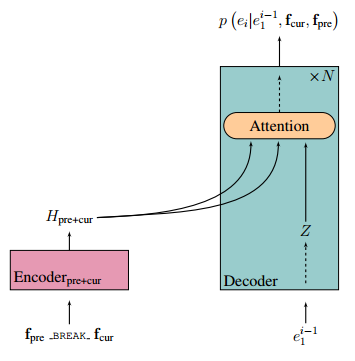
\includegraphics[width=0.45\linewidth]{Images/concatenation}
		\label{fig:concatenation}
	\end{figure}
\end{frame}

\begin{frame}{Concatenation Approaches}
For instance:
	\begin{itemize}
		\item<+(1)-|alert@+(1)> \cite{tiedemann_neural_2017} firstly introduced this approach proposing an \textbf{RNN-based} model that incorporate the preceding sentence by prepending it to the current one, separated by a $<$CONCAT$>$ token. They propose two methods:
			\begin{itemize}
				\item<+(1)-|alert@+(1)> \textbf{2-TO-2}: the previous and the current sentences are translated together. The translation of the current sentence is then obtained by only retaining the tokens following the concatenation token.
				\item<+(1)-|alert@+(1)> \textbf{2-TO-1}: only the current sentence is translated. 
			\end{itemize}
		\item<+(1)-|alert@+(1)> \cite{agrawal_contextual_2018,scherrer_analysing_2019} investigated the concatenation approach with the \textbf{Transformer} as base model, extending the number of context sentences both on the \textbf{source (s:-3,+1)} and the \textbf{target (t:-2)} side.
	\end{itemize}
\end{frame}

%%%%%%%%%%%%%%%%%%%%%%%%%%%%%%%%%%%%%%%%%%%%%%%%%%%%%%%%%%%%%%%%%%%%%%%%%
\subsection{Separate Encoding Approaches}

\begin{frame}{Separate Encoding Approaches}
Separate encoding approaches to DNMT consist in encoder-decoder models that encode the current and context sentences separately. This can be undertaken by:
	\begin{itemize}
		\item<+(1)-|alert@+(1)> \textbf{Multiple encoders} working in parallel for the current and previous sentence. E.g. \cite{wang_exploiting_2017}.
		\item<+(1)-|alert@+(1)> \textbf{Multiple encoders with shared weights}. In this case, the parallel-working encoders not only have the same architecture, but also the same weights. E.g. \cite{voita_context-aware_2018}.
		\item<+(1)-|alert@+(1)> \textbf{Two-pass approaches}, in which the encoder makes a first sentence-level encoding pass of the source, and a second in which it uses the context-agnostic drafts as contextual information for the current sentence. This can been achieved also by directly encoding the concatenation of many sentences and encoding them in a context-agnostic fashion, then encode context on top of it with extra layers. E.g. \cite{zheng_toward_2020}. See Slide \ref{slide:separateencoding}.
%		\begin{itemize}
%			\item<+(1)-|alert@+(1)> Remark: a powerful feature of two-pass approaches is their ability to exploit \textbf{future} target-side context.
%		\end{itemize}
	\end{itemize}  
\end{frame}

\begin{frame}{Separate Encoding Approaches}
Once the encoding of the current and the context sentences has been carried out, they can be integrated in different ways:
	\begin{columns}[T] % align columns
		\begin{column}{.50\textwidth}
			\begin{itemize}
				\item \textbf{Outside} the decoder. 
				\begin{itemize}
					\item (+) symbol represents a gate, a sum or a concatenation.
				\end{itemize}
			\end{itemize}
		\end{column}%
		\hfill%
		\begin{column}{.50\textwidth}
			\begin{figure}
				\centering
				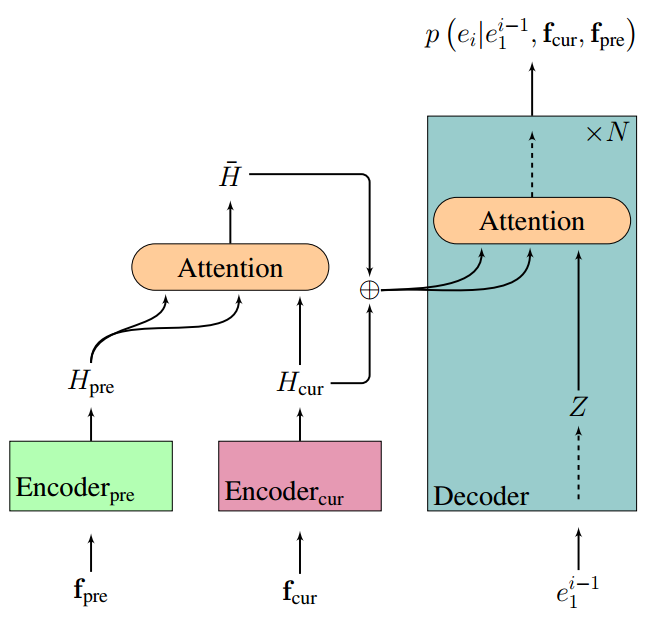
\includegraphics[width=0.90\linewidth]{Images/models_outide_decoder}
				\label{fig:modelsoutidedecoder}
			\end{figure}
		\end{column}%
	\end{columns} 
\end{frame}

\begin{frame}{Separate Encoding Approaches}
	Once the encoding of the current and the context sentences has been carried out, they can be integrated in different ways:
	\begin{columns}[T] % align columns
		\begin{column}{.50\textwidth}
			\begin{itemize}
				\item \textbf{Outside} the decoder.
					\begin{itemize}
						\item (+) symbol represents a gate, a sum or a concatenation.
					\end{itemize}
				\item \textbf{Inside} the decoder, \textbf{sequentially}. 
			\end{itemize}
		\end{column}%
		\hfill%
		\begin{column}{.50\textwidth}
			\begin{figure}
				\centering
				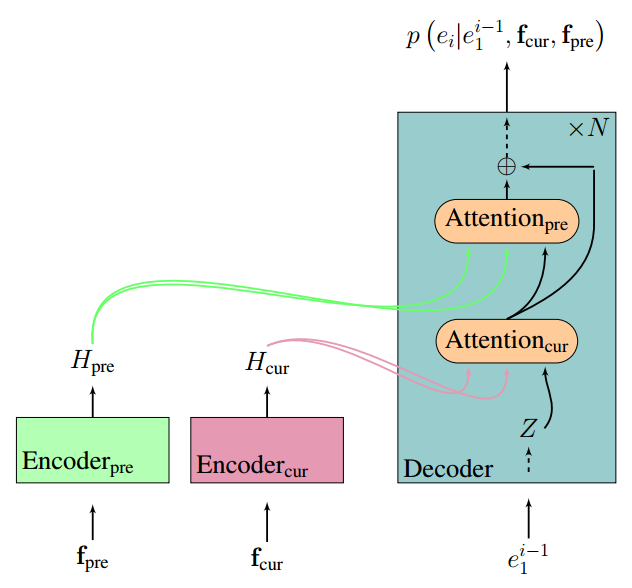
\includegraphics[width=0.90\linewidth]{Images/models_inside_decoder_sequential}
				\label{fig:modelsoutidedecoder}
			\end{figure}
		\end{column}%
	\end{columns} 
\end{frame}

\begin{frame}{Separate Encoding Approaches}
	Once the encoding of the current and the context sentences has been carried out, they can be integrated in different ways:
	\begin{columns}[T] % align columns
		\begin{column}{.50\textwidth}
			\begin{itemize}
				\item \textbf{Outside} the decoder.
					\begin{itemize}
						\item (+) symbol represents a gate, a sum or a concatenation.
					\end{itemize}
				\item \textbf{Inside} the decoder, \textbf{sequentially}.
				\item \textbf{Inside} the decoder, \textbf{in parallel}. 
			\end{itemize}
		\end{column}%
		\hfill%
		\begin{column}{.50\textwidth}
			\begin{figure}
				\centering
				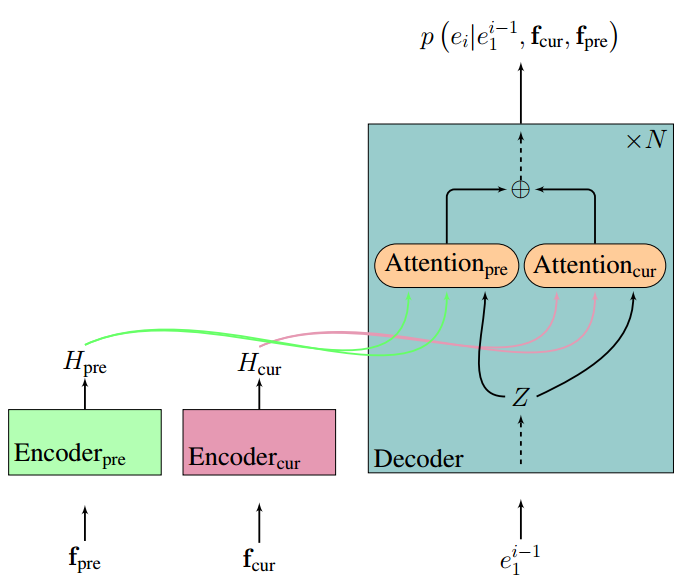
\includegraphics[width=0.90\linewidth]{Images/models_inside_decoder_parallel}
				\label{fig:modelsoutidedecoder}
			\end{figure}
		\end{column}%
	\end{columns} 
\end{frame}

%\begin{frame}{Separate Encoding Approaches}
%	\textbf{Architecture}\\
%	The encoder-decoder architectures depicted above can be both RNN-based (until 2017) or Transfomer-based (after 2017), as for any approach to DNMT. However, often some modifications are applied. For example:
%	\begin{itemize} 
%		\item<+(1)-|alert@+(1)> In the case of RNN-based architectures, integration inside the decoder can be undertaken without attention by simply concatenating context representations to the cell state of the deocdrr's RNN \cite{wang_exploiting_2017}.
%		\item<+(1)-|alert@+(1)>  Beside contextual representation of words, the context encoder can also generate higher level representations such as sentence or document embeddings. This representations can also be attended by the decoder \cite{miculicich_document-level_2018, maruf_selective_2019} or added to the word-representations \cite{tan_hierarchical_2019}.
%		\item<+(1)-|alert@+(1)> Parallel integration inside the decoder can also happen within a single multi-head attention that takes as values and queries the concatenations of the current and context sentence representations \cite{voita_when_2019}
%	\end{itemize}
%\end{frame}

\begin{frame}{Separate Encoding Approaches}
	\textbf{Including target-side context}\\
	Despite some have considered including past target-side context harmful because of the \textit{error propagation} problem \cite{zhang_improving_2018}, most recent works have showed it to be of utmost importance for making the most out of context. Past works have successfully included target-side context information in different ways:
	\begin{itemize}
		\item<+(1)-|alert@+(1)> Translating past sentences (usually 1) along with the current one, and then discarding them, as in concatenation approaches \cite{bawden_evaluating_2018}.
		\item<+(1)-|alert@+(1)> By making the decoder attend the target-side hidden representations or embeddings of previously decoded sentences \cite{miculicich_document-level_2018,voita_when_2019,maruf_selective_2019,zheng_toward_2020}.
	\end{itemize}
\end{frame}

\begin{frame}{Separate Encoding Approaches}\label{slide:separateencoding}
	\begin{table}
		\begin{tabular}{ *{5}{c|} c }

			\thead{Reference}
			& \thead{Context}
					& \thead{Two-Pass\\ Approach}
						& \thead{Outside\\ Integr.}
							& \thead{Inside\\ Integr.}
								& \thead{Lang.\\ Pair}
									 \\
			\hline\hline
			\cite{wang_exploiting_2017}&s:-3 &&aut...&...aut&Zh$\to$En\\
			\hline
			\cite{voita_context-aware_2018}&s:-1&&yes&&En$\to$Ru\\
			\hline
			\cite{zhang_improving_2018}&s:-2&&yes&sequential&Zh$\to$En\\
			\hline
			\cite{miculicich_document-level_2018}&s:-3; t:-3&&yes&&Zh/Es$\to$En\\
			\hline
			\cite{maruf_selective_2019}&s:all; t:all&optional&yes&&En$\to$De\\
			\hline
			\cite{zheng_toward_2020}&s:all; t:all&yes&yes&&Zh/En$\to$En/De\\
			\hline
			\cite{jean_does_2017}&s:-1&&&parallel&En$\to$De/Fr\\
			\hline
			\cite{bawden_evaluating_2018}&s:-1; t:-1&&&parallel&En$\to$Fr\\
			\hline
			\cite{fu_reference_2019}&s:all&yes&&parallel&En/Zh$\to$De/En\\
			\hline
			\cite{voita_when_2019}&s:-3; t:-3&yes&&parallel*&En$\to$Ru\\
			\hline
			\cite{tan_hierarchical_2019}&s:all&yes&&parallel&Zh/De$\to$En\\
			\hline
			\cite{wang_improving_2019} &s:2&&&sequential&Fr$\to$En\\
			\hline
		\end{tabular}
	\end{table}
\end{frame}

\begin{frame}{Positional Embedding Schema}
	For many approaches to DNMT, the standard positional encoding proposed by \cite{vaswani_attention_2017} is insufficient because the DNMT system needs to tell context sentences from the current one. For this reason, many strategies have been proposed in the literature, such as:
	\begin{enumerate}
		\item<+(1)-|alert@+(1)> Adding a \textbf{sentence distance embedding} to context sentences, that tell the model how far away they are from the current sentence \cite{voita_when_2019}.
		\item<+(1)-|alert@+(1)> Assign \textbf{positional embeddings progressively} to the current sentence, then to the previous one, and so on, so that far away sentences have high values of positional embedding \cite{li_pretrained_2019}.
		\item<+(1)-|alert@+(1)> Adding a \textbf{segment embedding}, similar to classical positional encoding but for the position of the sentence/segment within the document  \cite{zheng_toward_2020}.
	\end{enumerate}
\end{frame}

%%%%%%%%%%%%%%%%%%%%%%%%%%%%%%%%%%%%%%%%%%%%%%%%%%%%%%%%%%%%%%%%%%%%%%%%%
\subsection{Cache Approaches}

\begin{frame}{Cache Approaches}
	Cache approaches to DNMT consist in encoder-decoder models that are equipped with one or more caches that store context information.
	The information stored can belong to both \textbf{source side or target side, past and future}. 

	\begin{figure}
		\centering
		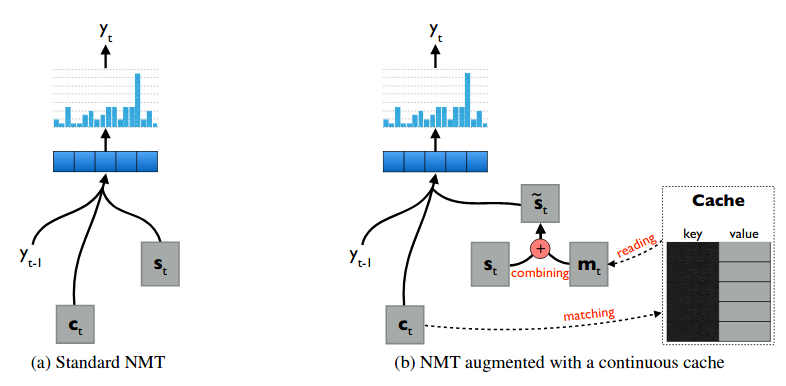
\includegraphics[width=0.7\linewidth]{Images/cache}
		\caption{Continuous cache by \cite{tu_learning_2017}}
		\label{fig:cache}
	\end{figure} 
\end{frame}

\begin{frame}[c]{Cache Approaches}
	\begin{columns}[c] % align columns
		\begin{column}{.50\textwidth}
			Every cache slot is a \textbf{key-value} tuple. With these variables, we can \textbf{read} or \textbf{write} caches.
			\vspace{0.3cm}
		\end{column}%
		\hfill%
		\begin{column}{.50\textwidth}
			\begin{figure}
				\centering
				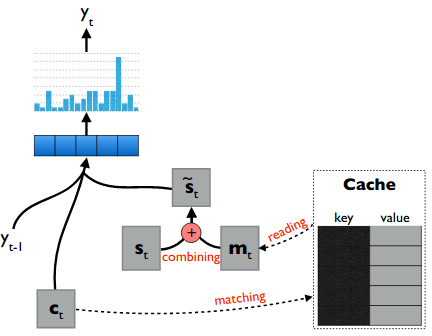
\includegraphics[width=0.9\textwidth]{Images/cache_only}
				\label{fig:cacheonly}
			\end{figure}
		\end{column}%
	\end{columns} 
\end{frame}

\begin{frame}[c]{Cache Approaches}
	\begin{columns}[c] % align columns
		\begin{column}{.50\textwidth}
			\textbf{Cache reading} involves:
			\begin{itemize}
				\item<+(1)-|alert@+(1)> Soft key matching
				\item<+(1)-|alert@+(1)> Value reading
				\item<+(1)-|alert@+(1)> Combining
			\end{itemize}
		\end{column}%
		\hfill%
		\begin{column}{.50\textwidth}
			\begin{figure}
				\centering
				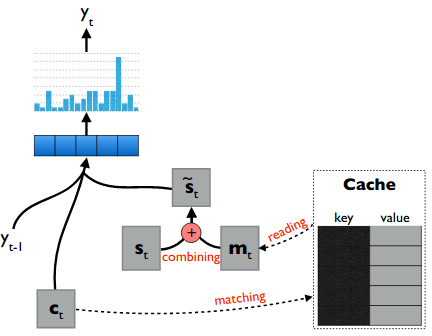
\includegraphics[width=0.9\textwidth]{Images/cache_only}
				\label{fig:cacheonly}
			\end{figure}
		\end{column}%
	\end{columns} 
\end{frame}

\begin{frame}{Cache Approaches}
	\begin{columns}[c] % align columns
		\begin{column}{.50\textwidth}
			\textbf{Cache writing} can be undertaken after having translated one or more sentences. For every triplet:
			\begin{itemize}
				\item<+(1)-|alert@+(1)> If the \textbf{key} already exists in the cache, we just update its value.  
				\item<+(1)-|alert@+(1)> Else, we write the key-value tuple in an empty slot, after having emptied the oldest slot if the cache is full.
			\end{itemize} 
		\end{column}%
		\hfill%
		\begin{column}{.50\textwidth}
			\begin{figure}
				\centering
				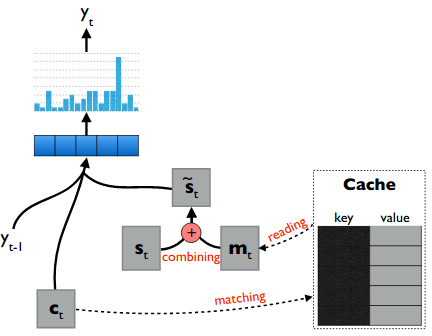
\includegraphics[width=0.9\textwidth]{Images/cache_only}
				\label{fig:cacheonly}
			\end{figure}
		\end{column}%
	\end{columns} 
\end{frame}

\begin{frame}{Cache Approaches}
	\begin{table}\small
	\begin{tabular}{p{3.6cm}|*{5}{c|} c }
		
		\thead{Reference}
		& \thead{Caches}
			& \thead{Size}
				& \thead{Key\\ (Indic.)}
					& \thead{Value}
							& \thead{Lang.\\ Pair}
		\\
		\hline\hline
		\cite{tu_learning_2017}&single&$\leq$ 500&$c_t$( $y_{k<t}$)&$s_{k<t}$&Zh$\to$En\\
		\hline
		\cite{kuang_modeling_2018}&\thead{dynamic\\ topic}&\thead{100\\ 200}&$c_t$&\thead{$y_{k<t}$\\ topic emb.}&Zh$\to$En\\
		\hline
		\cite{maruf_document_2018}&\thead{source\\ target}&\thead{doc.size}&\thead{$h_t$\\ $s_t$}&\thead{$sent. emb.$\\ $s_{k<t}$}&Fr/De/Et$\to$En\\
		\hline
	\end{tabular}
	\end{table}
\end{frame}

%%%%%%%%%%%%%%%%%%%%%%%%%%%%%%%%%%%%%%%%%%%%%%%%%%%%%%%%%%%%%%%%%%%%%%%%%
\subsection{Exploiting Document-level Monolingual Corpora}

\begin{frame}{On Parallel Corpora for Training}
	DNMT systems require training on \textbf{document-level parallel corpora}. These corpora are usually released during workshops on machine translation like IWSLT and WMT, and hosted on open source web inventories. The most common ones, are extracted from:
	\begin{itemize}
		\item<+(1)-|alert@+(1)> Movie subtitles (OpenSubtitles)
		\item<+(1)-|alert@+(1)> TED talks (WIT3)
		\item<+(1)-|alert@+(1)> News articles (LDC)
		\item<+(1)-|alert@+(1)> Parliamentary interventions (Europarl)
	\end{itemize}
\end{frame}

\begin{frame}{On Parallel Corpora for Training}
	\begin{itemize}
		\item<+(1)-|alert@+(1)> Unfortunately, document-level parallel \textbf{corpora are often insufficient} to train DNMT systems from scratch, although it is often possible to make them converge to a local optimum. 
		\item<+(1)-|alert@+(1)> \cite{kim_when_2019, li_does_2020} pointed out that when constraining training on such small datasets, model comparison becomes misleading because gains in performance are mainly related to better regularization.
		\item<+(1)-|alert@+(1)> A popular solution to this problem is the \textbf{two-step training strategy}: \cite{tu_learning_2017,zhang_improving_2018,miculicich_document-level_2018}
		\begin{enumerate}
			\item<+(1)-|alert@+(1)> Distinguish two integrated components in your model with params $\Theta=[\theta_S;\theta_D]$:
				\begin{itemize}
					\item<+(1)-|alert@+(1)> A self-standing sentence-level NMT system with parameters $\theta_S$.
					\item<+(1)-|alert@+(1)> Some context-handling modules with parameters $\theta_D$.
				\end{itemize}
			\item<+(1)-|alert@+(1)> Train $\theta_S$ independently on a sentence-level parallel corpus $C_S$.
			\item<+(1)-|alert@+(1)> Train $\theta_D$ on a document-level parallel corpus $C_D$ while fine-tuning $\theta_S$, or freezing them \cite{zhang_improving_2018}.
		\end{enumerate}
	\end{itemize}
\end{frame}

\begin{frame}{Exploiting Document-level Monolingual Corpora}
	Another solution to the lack of vast document-level parallel corpora is leveraging on huge \textit{monolingual} document-level corpora like BookCorpus \cite{zhu_aligning_2015} and PG-19 \cite{rae_compressive_2019}. In the literature, we can find various approaches to leverage monolingual corpora:
	\begin{itemize}
		\item<+(1)-|alert@+(1)> \textbf{Back-translate} target-side corpus to augment dl corpus \cite{sugiyama_data_2019}.
		\item<+(1)-|alert@+(1)> Train \textbf{context-aware language models} on target/source-side corpus, then:
		\begin{itemize}
			\item<+(1)-|alert@+(1)> Generate translations by fusioning the decoder and the LM's scores to candidate words  \cite{martinez_garcia_context-aware_2019}.
			\item<+(1)-|alert@+(1)> Initialize the econder (or decoder) of a DNMT model \cite{li_pretrained_2019}.
		\end{itemize}  
		\item<+(1)-|alert@+(1)> Train \textbf{Automatic Post Editing} systems on target-side corpus (See next slide).
	\end{itemize}
\end{frame}

\begin{frame}{Exploiting Document-level Monolingual Corpora}
	\textbf{Automatic Post Editing} (APE)\\
	\cite{voita_context-aware_2019} devised an APE system called DocRepair, that turns a sentence-level translation into a context-aware translation. DocRepair can work on top of whatever sentence-level MT system.
\end{frame}

\begin{frame}{DocRepair}
	\begin{columns}[c] % align columns
		\begin{column}{.50\textwidth}
			\begin{figure}
				\centering
				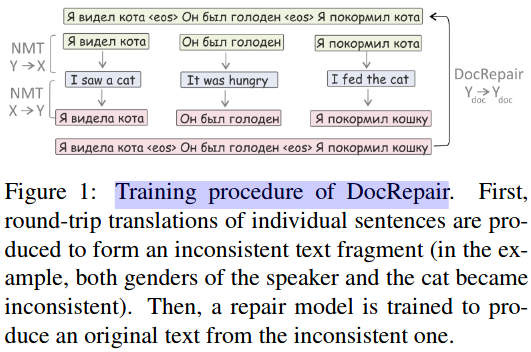
\includegraphics[width=\linewidth]{Images/docrepair_train}
				\label{fig:docrepairtrain}
			\end{figure}
		\end{column}%
		\hfill%
		\begin{column}{.50\textwidth}
			\begin{figure}
				\centering
				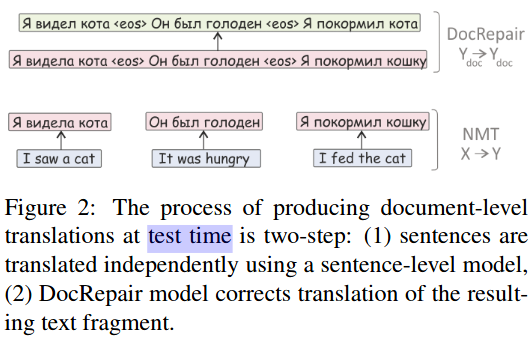
\includegraphics[width=\textwidth]{Images/docrepair_test}
				\label{fig:docrepairtest}
			\end{figure}
		\end{column}%
	\end{columns} 
\end{frame}

%%%%%%%%%%%%%%%%%%%%%%%%%%%%%%%%%%%%%%%%%%%%%%%%%%%%%%%%%%%%%%%%%%%%%%%%%
\subsection{Others}

\begin{frame}{Others}
	\textbf{Approaches Including Additional Discourse Information as Input}\\
	These approaches consist in concatenation approaches or separate encoding approaches that also integrate discourse-related information as additional input features. Examples of extra features are:
	\begin{itemize}
		\item<+(1)-|alert@+(1)> Lexical chains of semantically similar words to promote word sense disambiguation \cite{rios_gonzales_improving_2017}.
		\item<+(1)-|alert@+(1)> Coreference chains to promote coreference resolution \cite{stojanovski_coreference_2018, ohtani_context-aware_2019}.
	\end{itemize}
\end{frame}

\begin{frame}{Others}
	\textbf{Learning Approaches}\\
	 \cite{jean_context-aware_2019} looked at the problem from a learning perspective and designed a regularisation term
to encourage a DNMT model to exploit the additional context in a useful way . This regularisation
term is applied at the token, sentence and corpus levels and is based on pair-wise ranking loss,
that is, it helps to assign a higher log-probability to a translation paired with the correct context
than to the translation without context.
\end{frame}

%%%%%%%%%%%%%%%%%%%%%%%%%%%%%%%%%%%%%%%%%%%%%%%%%%%%%%%%%%%%%%%%%%%%%%%%%
\subsection{Remarks and conclusions}

\begin{frame}{Remarks and conclusions}
	\textbf{Possible Future Research Directions}
	\begin{itemize}
		\item<+(1)-|alert@+(1)> Build a large DL corpus for training systems, or find automatic approaches to generate synthetic data other than back-translation.
		\begin{itemize}
			\item<+(1)-|alert@+(1)> E.g. imputing context sentences \cite{jean_fill_2019}.
		\end{itemize}
%		\item<+(1)-|alert@+(1)> Design models with good results on lexical cohesion \cite{voita_when_2019}.
		\item<+(1)-|alert@+(1)> Design models exploiting full context in a memory-efficient way:
		\begin{itemize}
			\item<+(1)-|alert@+(1)> Dynamic context integration.
			\item<+(1)-|alert@+(1)> Caches integrated to Transformer-based models.
		\end{itemize}
		\item<+(1)-|alert@+(1)> Design automatic post-processing models that are lightweight and can be trained on little data \cite{kim_when_2019}.
		\item<+(1)-|alert@+(1)> Study pre-trained language models for DNMT decoder.
		\item<+(1)-|alert@+(1)> Study other learning methods that foster document-level modeling \cite{jean_context-aware_2019}.
	\end{itemize}
\end{frame}
%\section{Evaluation}

\begin{frame}{Evaluation}
	
	\begin{itemize}
		\item Classical metrics such as BLUE and METEOR are inadequate in evaluating document-level MT because they evaluate \textbf{average translation quality} at \textbf{sentence-level}. Thus:
		\begin{itemize}
			\item they are unable to capture document-wide phenomena like coherence and cohesion \cite{wong_extending_2012}
			\item they are not able to measure improvements over discourse phenomena that affect few words but heavily influence fluency and correctness of the translation \cite{muller_large-scale_2018}. E.g. pronomial anaphora.
		\end{itemize}
		\item Evaluation of \textbf{discourse phenomena} can be undertaken with:
			\begin{itemize}
				\item automatic metrics
				\item contrastive test suites
			\end{itemize}
	\end{itemize}

\end{frame}

\begin{frame}{Evaluation}
	
	\begin{figure}
		\centering
		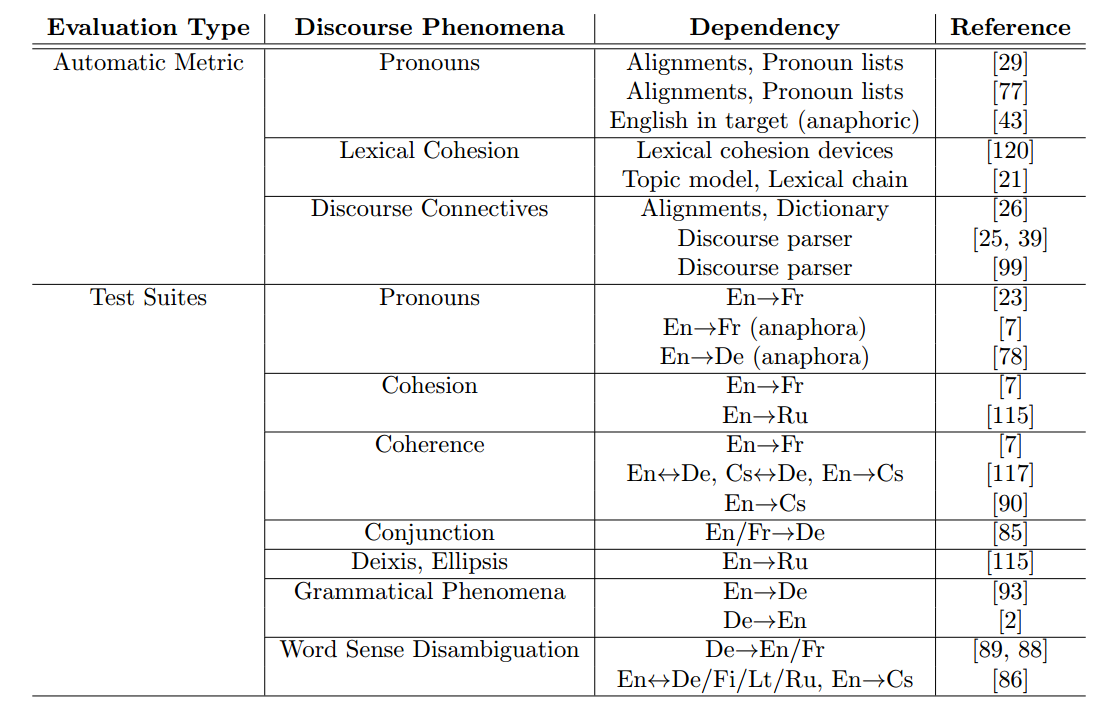
\includegraphics[width=0.7\linewidth]{Images/maruf_2019_discourse_phenomena}
		\caption{Overview of works on discourse phenomena evaluation in MT \cite{maruf_survey_2019}.}
			\label{fig:maruf2019discoursephenomena}
	\end{figure}
		
\end{frame}

\begin{frame}{Evaluation}
	
	
	\begin{itemize}
		\item The evaluation of discourse phenomena in document-level MT, \textit{desiderata}, and particularly the test suites, should:
		\begin{itemize}
			\item Provide inter-sentential context\footnote{in the remainder of this presentation, we refer to inter-sentential context simply as context.};
			\item Focus on context-dependent cases;
			\begin{itemize}
				\item E.g., pronominal anaphora cases in which the antecedent is in a previous sentence (context-dependent), instead of being in the same sentence (context-independent).
			\end{itemize}
			\item Focus on hard cases.
				\begin{itemize}
					\item E.g., when translating English to French, \textbf{he} is easy whereas \textbf{it} is hard to translate because ambiguous.
				\end{itemize}
		\end{itemize} 
	\end{itemize}
	
\end{frame}

\subsection{Automatic metrics}
\begin{frame}{Automatic metrics}

\textbf{Accuracy of Pronoun Translation} \cite{miculicich_werlen_validation_2017}:
	\begin{itemize}
		\item \textit{Compatible languages}: conceived for English to French but it has also been extended to other language pairs.
		\item \textit{Functioning}:
		\begin{itemize}
			\item Align source, reference and candidate translation with GIZA++ plus some heuristics;
			\item Compare candidate and reference pronouns taking into account \textbf{equivalent} pronouns and identical pronouns with \textbf{different forms} (target language-specific);
			\item E.g. \textit{it is difficult} $\rightarrow$ \textit{il/ce/c' est difficile}.
		\end{itemize}
	\end{itemize}

\end{frame}

\begin{frame}{Automatic metrics}
	
\textbf{Pronoun pair-wise ranking} \cite{jwalapuram_evaluating_2019}

\begin{itemize}
	\item \textit{Rationale1}: \textbf{ranking-based evaluation} measures can achieve higher correlations with human judgments, as rankings are simpler to obtain from humans and to train models on.
	\item \textit{Compatible languages}: all languages. The metric \textbf{only needs target-side inputs} $\implies$ thus it can be trained and evaluated without the need of a parallel corpus for each source-target pair.
	\item \textit{System input}: a pair $R=(C_r, r)$ and $S=(C_s, s)$ of translations to be compared, where:
	\begin{itemize}
		\item $C_r,C_s$ are the two translations. Each $C$ can comprise one or multiple sentences (context)
		\item $r,s$ are the positions of the pronouns to be compared in the translation $R$ and $S$, respectively.
	\end{itemize} 
\end{itemize}
	
\end{frame}


\begin{frame}{Automatic metrics}
	
\begin{figure}
	\centering
	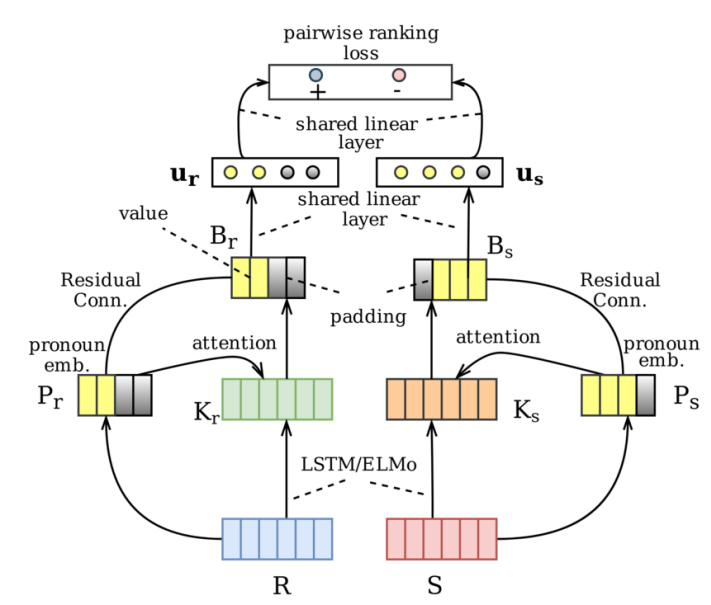
\includegraphics[width=0.55\linewidth]{Images/jwalapuram_2019_pronoun_ranker}
	\caption{Pairwise ranking system by \cite{jwalapuram_evaluating_2019}.}
	\label{fig:jwalapuram2019pronounranker}
\end{figure}

\end{frame}


\subsection{Test suites}
\begin{frame}{Test suites}
	
	\begin{itemize}
		\item \cite{bawden_evaluating_2018}: exemplary contrastive test suite, also good model reaching SOTA. Coherence very bad. Need for good models in coherence?
		\item \cite{muller_large-scale_2018}.  Proposal: A Large-Scale Test Set for the Evaluation of Context-Aware Pronoun Translation in Neural Machine Translation.
		\begin{itemize}
			\item Rationale: problems with previous contrastive test suites is that they are either too small to provide stathistical significance \cite{bawden_evaluating_2018} or not adapted to properly test DLNMT systems because lemmatized or not always with context.
			\item similar method will be adopted by \cite{jwalapuram_evaluating_2019}
			\item Focus: inter-sentential anaphora, hard case, , i.e., it → er, sie, es.
		\end{itemize}
	\end{itemize}
	
\end{frame}

\subsection{Remarks and conclusions}
\begin{frame}{Remarks and conclusions}
	
	\begin{itemize}
		\item automatic metrics
		\begin{itemize}
			\item are less expensive than human annotation and thus more easily applicable to all languages 
			\item are noisy because they often rely on other imperfect NLP systems. E.g. alignment and coreference systems.
			\item some automatic metrics might not be enough correlated with human judgment and miss the evaluation of some pronominal functions:
			\begin{itemize}
				\item is the case for APT, for example \cite{guillou_automatic_2018}
			\end{itemize}
			\item there is nothing on coherence although it's the most relevant for post-editors together with cohesion
		\end{itemize}
	
		\item test suites
		\begin{itemize}
			\item systems trained on in-domain data perform better?
		\end{itemize}

		\item what could we do?
		\begin{itemize}
			\item strongly test new automatic metrics against human judgment
			\item semi-automatic metrics: use a high precision automatic metric and a human to evaluate negative cases
			\item keep designing test suites for very restricted scope
		\end{itemize}
	\end{itemize}
	
\end{frame}



		


%\begin{itemize}[noitemsep,topsep=0pt]
%	\item<+(1)-|alert@+(1)> BLUE, METEOR, TER for average quality. Not good enough \cite{maruf_survey_2019}.
%	\item<+(1)-|alert@+(1)> \cite{bawden_evaluating_2018}: exemplary contrastive test suite, also good model reaching SOTA. Coherence very bad. Need for good models in coherence?
%\end{itemize}


\begin{frame}[c]{}
  \begin{center}
	  \Huge Thank you for your attention!
  \end{center} 
\end{frame}

%------------------------------------------------------------------------------
% Appendice
%------------------------------------------------------------------------------

\appendix
\backupbegin

\begin{frame}[allowframebreaks]
\frametitle{\refname}
%\nocite{*}
\bibliography{Bibliography/document_nmt}
\end{frame}

%\begin{frame}{Markov Decision Processes}
	\begin{block}{Reinforcement Learning}
		General class of algorithms that allow an agent to learn how to behave
		in a stochastic and possibly unknown environment by trial-and-error.
	\end{block}
	
	\begin{block}{Markov Decision Process (MDP)}
		stochastic dynamical system specified by $<\S, \A, \calP, \calR, \gamma>$
		\begin{enumerate}
			\item $(\S, \calS)$ is a measurable state space
			\item $(\A, \calA)$ is a measurable action space
			\item $\calP: \S \times \A \times \calS \to \R$ is a Markov transition kernel
			\item $\calR: \S \times \A \to \R$ is a reward function
			\item $0 < \gamma < 1$ is the discount factor.
		\end{enumerate}
	\end{block}
\end{frame}



\begin{frame}{Monte-Carlo Policy Gradient: Pseudocode}
	\begin{algorithmic}[1]
		\Require Stochastic policy $\pi_\theta$, Initial parameters $\theta_0$, learning rate $\{\alpha_k\}$
		\Ensure Approximation of the optimal policy $\pi_{\theta^*} \approx \pi_*$
		\Repeat
			\State Sample $M$ trajectories $h^{(m)} = \{(s_t^{(m)}, a_t^{(m)}, r_{t+1}^{(m)})\}_{t = 0}^{T^{(m)}}$ under policy $\pi_{\theta_k}$   
			\State Approximate policy gradient 
			\begin{equation*}
				\nabla_\theta J(\theta_k) \approx \frac{1}{M} \sum_{m=0}^M
				 \sum_{u=0}^{T^{(m)}-1} \nabla_\theta\log \pi_{\theta_k} \left(s_u^{(m)}, a_u^{(m)}\right) 
				 \sum_{v \geq u}^{T^{(m)}-1} \gamma^{v-u} r_{v+1}^{(m)}   
			\end{equation*}
			\State Update parameters using gradient ascent $\theta_{k+1} = \theta_k + \alpha_k \nabla_\theta J(\theta_k)$
			\State $k \leftarrow k + 1$
		\Until{converged}
	\end{algorithmic}
\end{frame}


\begin{frame}{Episodic PGPE Algorithm: Pseudocode}
	\begin{algorithmic}[1]
		\Require Controller $F_\theta$, hyper-distribution $p_\xi$, initial guess $\xi_0$, learning rate $\{\alpha_k\}$
		\Ensure Approximation of the optimal policy $F_{\xi^*} \approx \pi_*$
		\Repeat
			\For {$m = 1, \ldots, M$}
				\State Sample controller parameters $\theta^{(m)} \sim p_{\xi_k}$ 
				\State Sample trajectory $h^{(m)} = \{(s_t^{(m)}, a_t^{(m)}, r_{t+1}^{(m)})\}_{t = 0}^{T^{(m)}}$ under policy $F_{\theta^{(m)}}$
			\EndFor
			\State Approximate policy gradient 
		  		\begin{equation*}
		  		\nabla_\xi J(\xi_k) \approx \frac{1}{M} \sum^{M}_{m=1} \nabla_\xi \log p_\xi\left(\theta^{(m)}\right) \left[G\left(h^{(m)}\right)-b\right] 
		  		\end{equation*}
		  		
			\State Update hyperparameters using gradient ascent $\xi_{k+1} = \xi_k + \alpha_k \nabla_\xi J(\xi_k)$
			\State $k \leftarrow k + 1$
		\Until{converged}
	\end{algorithmic}
\end{frame}

\begin{frame}{Truncated Multiple Importance Sampling Estimator}

\begin{block}{Importance Sampling}
Given a bounded function $f:\mathcal{Z}\to\Reals$, and a set of \iid outcomes $z_1,\dots,z_N$ sampled from $Q$, the importance sampling estimator of $\mu:=\Exp_{z\sim P}\left[f(z)\right]$ is:
\begin{equation}\label{eq:ise}
	\wh{\mu}_{\text{IS}} = \frac{1}{N}\sum_{i=1}^{N}f(z_i)w_{P/Q}(z_i),
\end{equation}
which is an unbiased estimator, \ie ${\Exp_{z_i\simiid Q}\left[\wh{\mu}_{IS}\right] = \mu}$.
\end{block}

\begin{block}{Truncated Estimator With Balance Heuristic}
\begin{equation}\label{eq:truncatedmise}
	\widecheck{\mu}_{\text{BH}} =\frac{1}{N} \sum_{k=1}^K\sum_{i=1}^{N_k} \min \left\{M,  \frac{p(z_{ik})}{\sum_{j=1}^K \frac{N_j}{N} q_j(z_{ik})} \right\} f(z_{ik}).
\end{equation}
\end{block}

\end{frame}

\begin{frame}{OPTIMIST2}
\begin{theorem}{regretdiscretized}\label{th:regretdiscretized}
	Let $\Xspace$ be a $d$-dimensional compact arm set with $\Xspace \subseteq [-D,D]^d$. For any $\kappa\geq2$, under Assumptions 1 and 2, OPTIMIST2 with confidence schedule ${\delta_t = \frac{6\delta}{\pi^2t^2\left(1+\left\lceil t^{\nicefrac{1}{\kappa}}\right\rceil^d\right)}}$ and discretization schedule $\tau_t=\lceil t^{\frac{1}{\kappa}} \rceil$ guarantees, with probability at least $1-\delta$:
	\begin{align*}
	&\Reg(T) \leq \Delta_0  + C_1T^{\left(1-\frac{1}{\kappa}\right)}d
	+ C_2
	T^{\frac{1}{1+\epsilon}} %\,\cdot
	\\&\quad\cdot\left[v_{\epsilon}
	\left(\left(2+ \nicefrac{d}{\kappa}\right)\log T + d\log 2 + \log\frac{\pi^2}{3\delta}\right)\right]^{\frac{\epsilon}{1+\epsilon}},
	\end{align*}
	where $C_1=\frac{\kappa}{\kappa-1}LD$, $C_2=(1+\epsilon)\left(2\sqrt{2}+\frac{5}{3}\right)\norm[\infty]{f}$, and $\Delta_0$ is the instantaneous regret of the initial arm $\vx_0$.
\end{theorem}
\end{frame}

\backupend

\end{document}
